%% Type de document et encodage de la police
\documentclass[a4paper]{article}
\usepackage[utf8x]{inputenc}
\usepackage[T1]{fontenc}
% \usepackage[french]{babel}

%% Initialise la taille des pages et des marges
\usepackage[a4paper, top=3cm, bottom=3cm, left=2cm, right=2cm, marginparwidth=2cm]{geometry}

%% import tex documents
\usepackage[subpreambles=true]{standalone}
\usepackage{import}

%% Packs utiles
\usepackage{amsmath}
\usepackage{graphicx}
\usepackage{xcolor}
\usepackage{textcomp}

%% Commandes perso
\renewcommand{\arraystretch}{1.2} %% row 20% longer
\definecolor{sprinen}{rgb}{0.0, 1.0, 0.7}

%% Pour les exemples
\usepackage{mdframed}
\newmdenv[topline=false, bottomline=false, rightline=false, skipabove=\topsep, skipbelow=\topsep]{example}

%% Pour les diagrammes
\usepackage{tikz}


\title{Sécurité \& Bien-Être en Milieu Professionnel}
\author{Grégoire Roumache}
\date{Décembre 2019}

\begin{document}

\maketitle





20 questions à l'examen,
\begin{itemize}
    \item 10 à 15 questions sur le tome n\textdegree1,
    \item 3 à 6 questions sur le tome n\textdegree2,
    \item 2 à 4 questions sur le tome n\textdegree3.
\end{itemize}










\section{Tome n\textdegree1}










\subsection{Cadre historique et légal}





\begin{itemize}





\item Cadre historique \& légal:
\begin{center}
    \begin{tabular}{|l|p{8cm}|} \hline
        en 1789 & révolution française \\ \hline
        vers 1888 & Naissance de la lutte syndicale en Belgique \\ \hline
        vers 1950 & Écriture du RGPT \\
        & (Obligation de moyens) \\ \hline
        en 1996 & Écriture du Code du Bien-Être \\
        & (Loi du 4 août 1996 et obligation de résultats) \\ \hline
    \end{tabular}
\end{center}
Remarques:
\begin{itemize}
    \item RGPT = Règlement Général pour la Protection du Travail
    \item \textbf{Réglement} = obligation de \textbf{moyens}
    \item \textbf{Code} = obligation de \textbf{résultats}
\end{itemize}





\item Objectifs principaux de la législation sur le bien-être au travail:
\begin{itemize}
    \item \textbf{Protéger les travailleurs} et d’autres personnes lors de l’exécution des travaux.
    \item \textbf{Améliorer la sécurité et la santé} au travail des travailleurs.
    \item Assurer des \textbf{conditions de travail} aussi \textbf{bonnes} que possible.
\end{itemize}





\item \textcolor{red}{\textbf{Q. d'examen:}} Qu'est-ce qu'un travailleur ?
\begin{center}
    \textcolor{blue}{\textbf{Travailleurs = ouvriers, cadres, bénévoles, stagiaires, ...}}
\end{center}
Remarques:
\begin{itemize}
    \item La loi sur le travail est d’application pour des travaux réalisés dans l'entreprise (ex: ateliers, bureaux);
    \item mais aussi pour les travaux réalisés en dehors de l’entreprise (ex: chez un client).
    \item Peu importe si le lieu de travail est un espace clos ou ouvert.
\end{itemize}





\item Principes de base:
\begin{enumerate}
    \item \textbf{Employeurs \& travailleurs} ont des \textbf{droits et des obligations} en matière de sécurité et de santé.
    \item L’\textbf{employeur} est \textbf{responsable} et mène une politique de bien-être au travail.
    \item Cette \textbf{politique} est \textbf{basée sur la prévention des risques}.
    \item Le travail ne peut \textbf{pas} avoir \textbf{un effet négatif sur la sécurité et la santé des travailleurs}.
    \item L’employeur se fait \textbf{assister par des experts} (services de prévention).
    \item L’\textbf{information et} la \textbf{formation} des travailleurs.
    \item \textbf{Consultation et collaboration} avec les travailleurs et/ou leur représentation.
    \item \textbf{Les employeurs} qui travaillent \textbf{sur un même lieu} doivent se \textbf{coordonner et collaborer}.
\end{enumerate}





\item \textcolor{red}{\textbf{Attention !}} 7 domaines du bien-être:
\begin{enumerate}
    \item \textbf{Sécurité au travail}: éviter les accidents.
    \item \textbf{Santé au travail}: prévention des maladies.
    \item \textbf{Charge psychosociale}: prévenir le stress négatif, la violence, le harcèlement moral et sexuel.
    \item \textbf{Ergonomie}: poste de travail adapté au travailleur.
    \item \textbf{Hygiène au travail}: limiter l'exposition au bruit, vibrations, substances dangereuses, etc.
    \item \textbf{Embellissement des lieux de travail}:
    \begin{itemize}
        \item lieu de travail agréable et soigné (idem pour les sanitaires, réfectoires, etc.)
        \item possibilités suffisantes pour se laver (douches, vestiaires, etc.)
    \end{itemize}
    \item \textbf{Environnement}: collecte, traitement des déchets; entreposage adéquat des substances dangereuses.
\end{enumerate}
Remarques:
\begin{itemize}
    \item \textbf{risque} psychologique $ \neq $ \textbf{charge} psychologique
    \item harcèlement $ \implies $ côté répétitif
    \item Risque psychologique:
    \begin{itemize}
        \item harcèlement moral/sexuel
        \item burn-out
        \item violences verbales/physiques
        \item discriminations
    \end{itemize}
\end{itemize}





\item Schéma sécurité entreprise:
\begin{center}
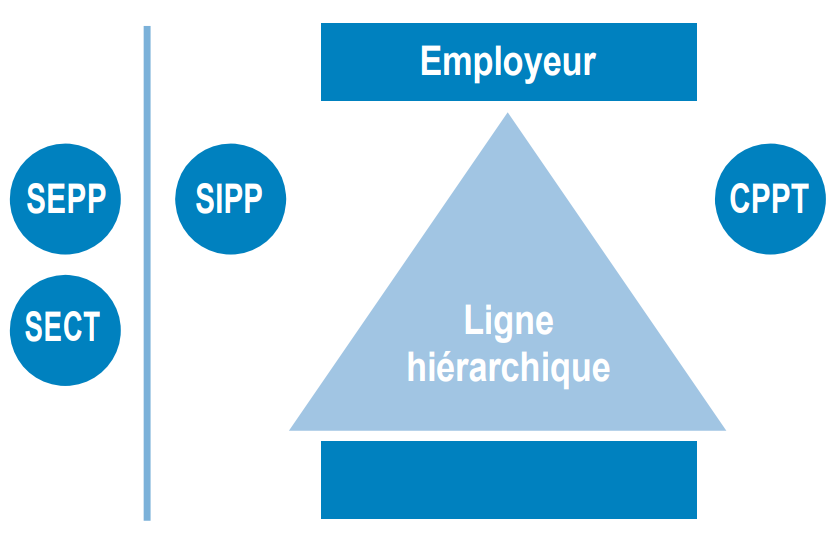
\includegraphics[width=0.5\textwidth]{images/schema-entreprise.PNG}
\end{center}
Acronymes:
\begin{itemize}
    \item SEPP = Service Externe pour la Prévention et la Protection au travail
    \item SIPP = Service Interne pour la Prévention et la Protection au travail
    \item SECT = Service Externe de Contrôle Technique
    \item CPPT = Comité pour la Prévention et la Protection au Travail
\end{itemize}





\item Services de prévention:
\begin{itemize}
    \item chaque entreprise doit constituer un service interne de prévention/protection au travail,
    \item si l'entreprise a moins de 20 travailleurs, l'employeur peut exercer lui-même cette fonction,
    \item l’entreprise doit faire appel à un service externe pour les compétences qu'elle ne posssède pas.
\end{itemize}
Tâches des conseillers en prévention:
\begin{itemize}
    \item analyser les risques (= inventaire \& évaluation des risques),
    \item analyser les accidents \& presqu'accidents,
    \item réaliser la surveillance de santé (conseillers en prévention, médecins de travail)
    \item rendre des avis à l'employeur \& aux travailleurs
    \begin{example}
        "rendre un avis": le travailleur se décharge de sa responsabilité si il dit que le sol est glissant par exemple.
    \end{example}
\end{itemize}





\item L'employeur doit prévoir une \textbf{formation}, une \textbf{information} et un \textbf{accueil} suffisants et adéquats:
\begin{enumerate}
    \item avant de commencer à travailler,
    \item en cas de mutation/changement de poste,
    \item lors d'un changement d'équipement de travail,
    \item lors de l’introduction de nouveaux procédés de travail (ex: nouvelles technologies).
\end{enumerate}





\item Les \textbf{inspecteurs} peuvent prendre les mesures suivantes:
\begin{itemize}
    \item Donner des avertissements et des conseils.
    \item Imposer des mesures et des délais pour se conformer à la législation.
    \item Faire arrêter immédiatement le travail en cas de danger imminent pour des personnes et éventuellement faire évacuer le lieu de travail.
    \item Dresser un procès-verbal en cas d’infraction.
\end{itemize}





\item Hiérarchie des sources de droit:
\begin{enumerate}
    \item \textbf{directives européennes},
    \item transposition en \textbf{droit belge}, sous forme de lois qui définissent les principes généraux,
    \item la loi est mise en application par ses \textbf{arrêtés royaux et ministériels}.
\end{enumerate}





\item Cadre général de la législation:
\begin{enumerate}
    \item Droit international
    \item Organisation internationale du Travail (OIT)
    \item Le Conseil de l’Europe
    \item L’Union européenne
    \item La Constitution belge
    \item La Loi et ... les AR qui en découlent \textcolor{red}{\textbf{Attention ! Les (...) sont très importants. Q. d'examen...}}
    \item Les décrets et les ordonnances des Communautés et des Régions
\end{enumerate}





\item Cadre national de la législation:
\begin{enumerate}
    \item Un \textbf{arrêté royal} (AR) est une décision du Roi. Tout acte du Roi doit être contresigné par au moins un ministre, qui en prend la responsabilité devant le Parlement.
    \item Les \textbf{arrêtés-lois} et les \textbf{arrêtés royaux de pouvoirs spéciaux} sont des décisions prises par le Roi sur la base d’une délégation de pouvoirs du Parlement.
    \item Les \textbf{arrêtés ministériels} sont des décisions d’un ministre. La constitution n’accorde aux ministres aucune compétence réservée, ce sont donc des mesures d’application de lois et d’arrêtés royaux, auxquels ils doivent se conformer.
    \item Les \textbf{circulaires ministérielles} et les \textbf{instructions administratives} sont des ordres/recommandations pour les fonctionnaires. Elles ne lient ni les citoyens, ni les tribunaux, mais elles ont une certaine autorité d’influence.    
    \item La \textbf{convention collective de travail} est un accord entre une (ou plusieurs) organisation représentative des travailleur, et soit un (ou plusieurs) employeur/organisation d’employeurs.
    \item Le \textbf{règlement de travail} est une sorte de règlement d’ordre intérieur de l’ entreprise. Chaque entreprise doit en avoir un et chaque employé doit en recevoir une copie.
\end{enumerate}





% \item Hiérarchie des sources du droit social:
% \begin{enumerate}
%     \item (le droit international et la constitution) - les dispositions impératives de la loi,
%     \item Les conventions collectives rendues obligatoires, selon l’ordre suivant:
%     \begin{enumerate}
%         \item convention du CNT (= Conseil National du Travail)
%         \item convention d’une commission paritaire
%         \item convention d’une sous-commission paritaire
%         \item conventions collectives non rendues obligatoires
%         \item contrat de travail écrit
%         \item conventions collectives conclues au sein d’un organe paritaire et non-rendues
%         \item règlement de travail
%         \item dispositions supplétives de la loi
%         \item contrat de travail verbal
%         \item l'usage...
%     \end{enumerate}
% \end{enumerate}





\item \textbf{Définition jurisprudence}: On appelle jurisprudence la façon dont les tribunaux jugent habituellement une question donnée. \\
Remarques:
\begin{itemize}
    \item En Belgique, la jurisprudence n’est pas une source obligatoire du droit.
    \item Toutefois, la jurisprudence a une grande autorité d’influence, surtout celle des cours supérieures.
\end{itemize}





\item Organisation du pouvoir judiciaire en Belgique:
\begin{center}
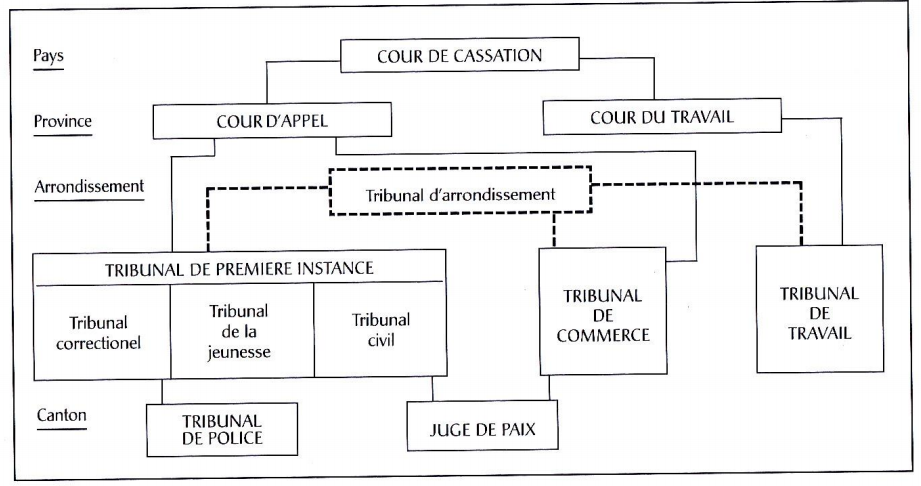
\includegraphics[width=0.65\textwidth]{images/organisation-judiciaire.PNG}
\end{center}





\item Le travailleur a droit à:
\begin{itemize}
    \item un environnement de travail sécurisé et sain,
    \item l'information (via la fiche de travail notamment) et à la formation,
    \item l'interruption du travail en cas de danger imminent et grave pour les personnes.
\end{itemize}





\item Obligations du travailleur:
\begin{enumerate}
    \item veiller à votre propre sécurité et à celle des autres,
    \item utiliser correctement et en toute sécurité les outils, machines, etc.,
    \item utiliser correctement les équipements de protection individuelle et en prendre soin,
    \item suivre les consignes, instructions et informations de sécurité reçues,
    \item signaler les situations dangereuses, accidents, quasi-accidents au supérieur et intervenir de manière appropriée,
    \item ne pas désactiver les dispositifs de sécurité des outils, machines, etc. et ne pas modifier ou déplacer ces dispositifs mais les utiliser de manière adéquate,
    \item signaler immédiatement les manquements ou erreurs dans les systèmes de protection,
    \item collaborer de manière positive à la politique de prévention de l’employeur, par exemple en donnant votre opinion sur les risques inhérents à votre tâche,
    \item collaborer avec le service de prévention et protection au travail,
    \item prendre part aux informations, formations, exercices de votre employeur,
    \item s'abstenir de toute forme de violence, brimade ou harcèlement moral et sexuel au travail.
\end{enumerate}





\item Objectif de la fiche de poste de travail = échanger des informations concernant:
\begin{enumerate}
    \item le poste à pourvoir,
    \item les risques de ce poste de travail pour la sécurité \& la santé,
    \item les mesures de prévention à prendre.
\end{enumerate}





\end{itemize}










\subsection{Domaines du bien-être}





\begin{itemize}





\item Il existe différents type d’examens médicaux:
\begin{itemize}
    \item \textbf{avant de travailler} ou lors d’un changement de fonction,
    \item \textbf{périodique} pour des catégories à risque (par rapport au règlement et la fonction),
    \item \textbf{après une longue absence} (4 semaines) pour maladie ou accident.
\end{itemize}





\item Notions de risque \& de danger:
\begin{itemize}
    \item danger = caractéristique intrinsèque d’un produit ou situation pouvant provoquer des dommages
    \item risque = degré de probabilité qu’un danger provoque un évènement avec dommage
\end{itemize}





\item Le système dynamique de gestion des risques se compose d’étapes successives:
\begin{itemize}
    \item Objectifs et élaboration de la politique et des mesures.
    \item Planning et programmation.
    \item Mise en oeuvre.
    \item Suivi et évaluation.
    \item Adaptation.
\end{itemize}





\item Cercle de Deming (= étapes dans la gestion des risques):
\begin{center}
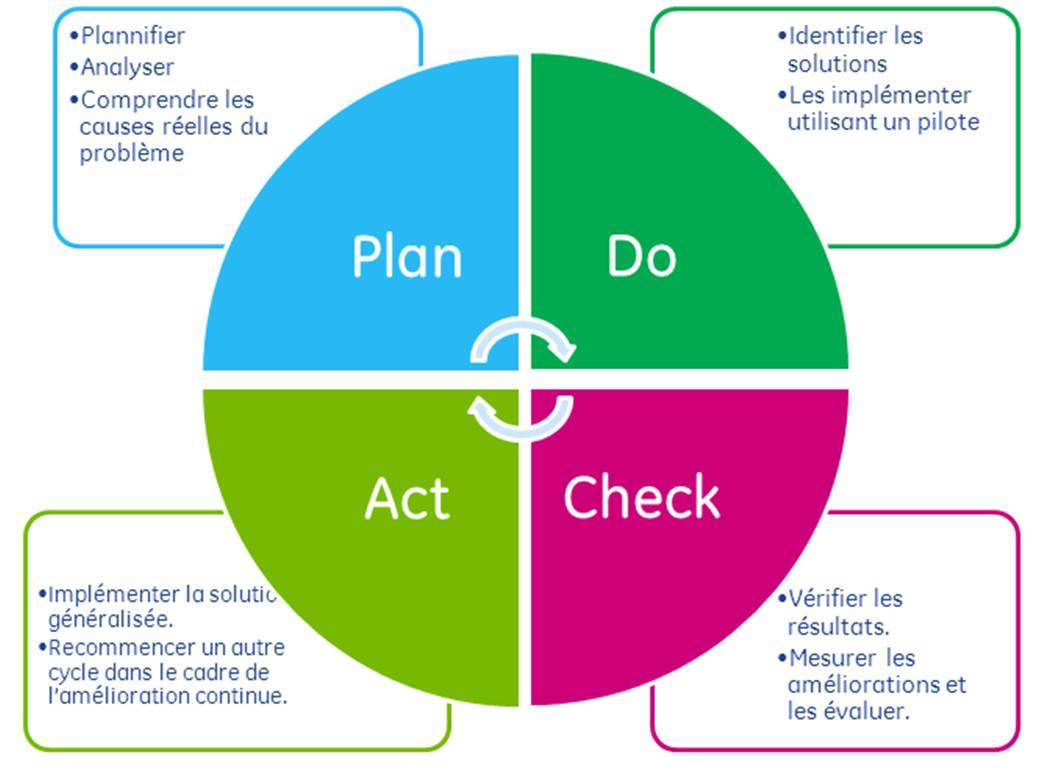
\includegraphics[width=0.75\textwidth]{images/cercle-deming.jpg}
\end{center}





\item Analyse générale des risques:
\begin{enumerate}
    \item Identification des dangers.
    \item Identification/détermination des risques.
    \begin{example}
        Les dangers posent-ils un risque au travailleur ? \\
        Des lésions ou des dégâts peuvent-ils se produire ?
    \end{example}
    \item Évaluation des risques.
    \begin{example}
        Quelle peut être la gravité des conséquences ? \\
        Quelle est la probabilité que ces conséquences (blessures, dommage) surviennent ?
    \end{example}
\end{enumerate}





\item Le risque sous forme de formule:
\begin{center}
    Risque = probabilité $ \times $ effet \\
    R = (P $ \times $ F) $ \times $ E
\end{center}
Abréviations:
\begin{itemize}
    \item R = risque
    \item P = probabilité
    \item F = fréquence d'exposition
    \item E = ampleur des dommages éventuels (gravité)
\end{itemize}





\item Notions d’accidents, d’incidents:
\begin{center}
\begin{tikzpicture}
    \node [anchor=west] at (0,0) {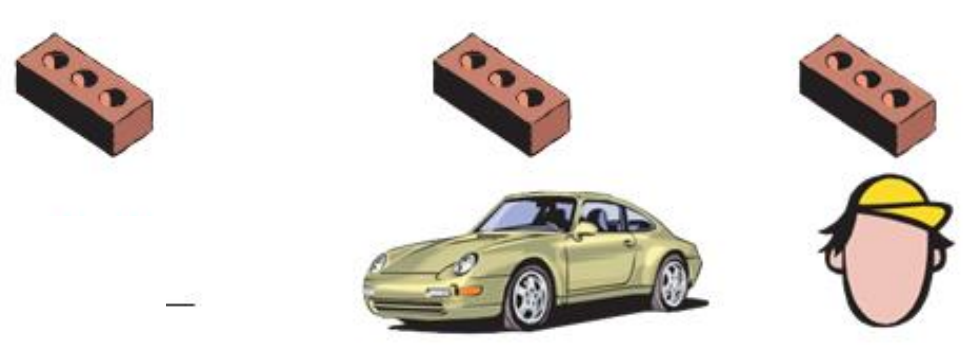
\includegraphics[width=9cm]{images/accident-incident.PNG}};
    \node [] at (1,-2) {danger};
    \node [] at (8.25,-2) {accident};

    \draw (0,-2.55) -- (0,-2.8) -- (7.25,-2.8) -- (7.25,-2.55);
    \node [] at (3.75,-3.25) {incidents};
\end{tikzpicture}
\end{center}





\item \textcolor{red}{\textbf{Attention !}} Notion d'accident du travail -- éléments constitutifs:
\begin{enumerate}
    \item sur le lieu du travail,
    \item par le fait du travail,
    \item lors de l'exécution du travail,
    \item lésion,
    \item plus d'un jour d'absence.
\end{enumerate}
Remarque: l'accident est un \textbf{événement soudain}, c'est ce qui le distingue d'une maladie.





\item Taux de fréquence \& Taux de gravité:
\begin{itemize}
    \item Taux de fréquence (Tf) = nombre d’accidents pendant une période déterminée.
    \item Taux de gravité réel (Tg) = gravité des accidents pendant une période déterminée. \\
    C’est l’absence au travail, l’incapacité temporaire, qui est prise en compte.
\end{itemize}





\item Notions d’absentéisme:
\begin{itemize}
    \item \textbf{Absentéisme noir}: se déclarer malade sans être malade.
    \item \textbf{Absentéisme gris}: se déclarer malade parce que l'on se sent malade sans être vraiment malade.
    \item \textbf{Absentéisme blanc}: se déclarer malade et être malade.
\end{itemize}





\item Il existe une liste de maladies professionnelles. Si votre maladie n'est pas dans la liste, il faut prouver un lien de causalité entre la profession et la maladie. \\
Exemples de maladies professionnelles:
\begin{itemize}
    \item syndrôme du canal carpien
    \item asbestose, maladie due à la présence de l'amiante (asbeste = amiante)
\end{itemize}





\item \textcolor{red}{\textbf{Attention !}} Hiérarchie de prévention:
\begin{enumerate}
    \item éliminer le risque (combattre les risques à la source)
    \item limiter ou réduire le risque (protection collective) (EPC)
    \item équipements de protection individuelle (EPI)
    \item information
\end{enumerate}
Remarques:
\begin{itemize}
    \item EPC = équipement de protection collective
    \item EPI = équipement de protection individuelle
\end{itemize}





\item Quelles sont les conditions auxquelles les EPI doivent répondre ?
\begin{itemize}
    \item Porter un marquage CE.
    \item Être adaptés aux conditions de travail.
    \item Être adaptés au risque spécifique et offrir une protection suffisante.
    \item Ne pas entraîner de nouveaux risques pour l’utilisateur, et ne pas le gêner.
    \item Correspondre à la taille de l’utilisateur, être réglables ou faits sur mesure.
\end{itemize}





\item Notion de décibel: niveau d’intensité (ou niveau sonore) d’une onde acoustique se définit comme le nombre de multiplications par 10 nécessaire pour obtenir sa valeur à partir du seuil d’audibilité.
\[ \beta = 10 \log \frac{I}{I_0} = 20 \log \frac{P}{P_0} \]





\item Règles de calcul \& formules:
\begin{center}
\begin{tabular}{ll}
    P $ \times $ 2  & dB + 3 \\
    P $ \div $ 2  & dB - 3 \\
    P $ \times $ 10  & dB + 10 \\
    P $ \div $ 10  & dB - 10
\end{tabular}
\end{center}
\[ \text{intensité} \approx \text{dist}^2 \qquad  \implies  \qquad \text{dist} \approx \sqrt{\text{intensité}} \]





\item \textcolor{red}{\textbf{Attention !}} Protection auditive: àpd 80 décibels des lésions auditives peuvent survenir.
\begin{itemize}
    \item Lorsque des travailleurs sont exposés, pendant 8h supérieur à cette limite, l’employeur doit mettre des protections auditives à disposition.
    \item Lorsque le niveau sonore atteint 85 dB(A), la protection auditive est obligatoire.
\end{itemize}





\item \textcolor{blue}{Avoir une bonne vue plus longtemps}: prendre des pauses toutes les 30 minutes et de regarder au loin afin de reposer nos yeux.





\item \textcolor{red}{\textbf{Attention ! Q. d'examen.}} Principes de précaution du non-filaire par rapport au filaire (non-filaire = wifi):
\begin{enumerate}
    \item Principe de justification
    \item Principe d’optimisation
    \item Principe de non-accumulation
\end{enumerate}





\item Filtres à poussières:
\begin{center}
    \begin{tabular}{|l|l|} \hline
        P1 & Protection contre les poussières irritantes \\ \hline
        P2 & Protection contre les poussières nocives \\ \hline
        P3 & Protection contre les poussières toxiques \\ \hline
    \end{tabular}
\end{center}
Remarques:
\begin{itemize}
    \item P pour "particule"
    \item chiffre élevé = meilleure capacité de rétention de la poussière (car + dangereux)
\end{itemize}





\item \textcolor{red}{\textbf{Attention !}} Pictogrammes sur les vêtements de protection:
\begin{center}
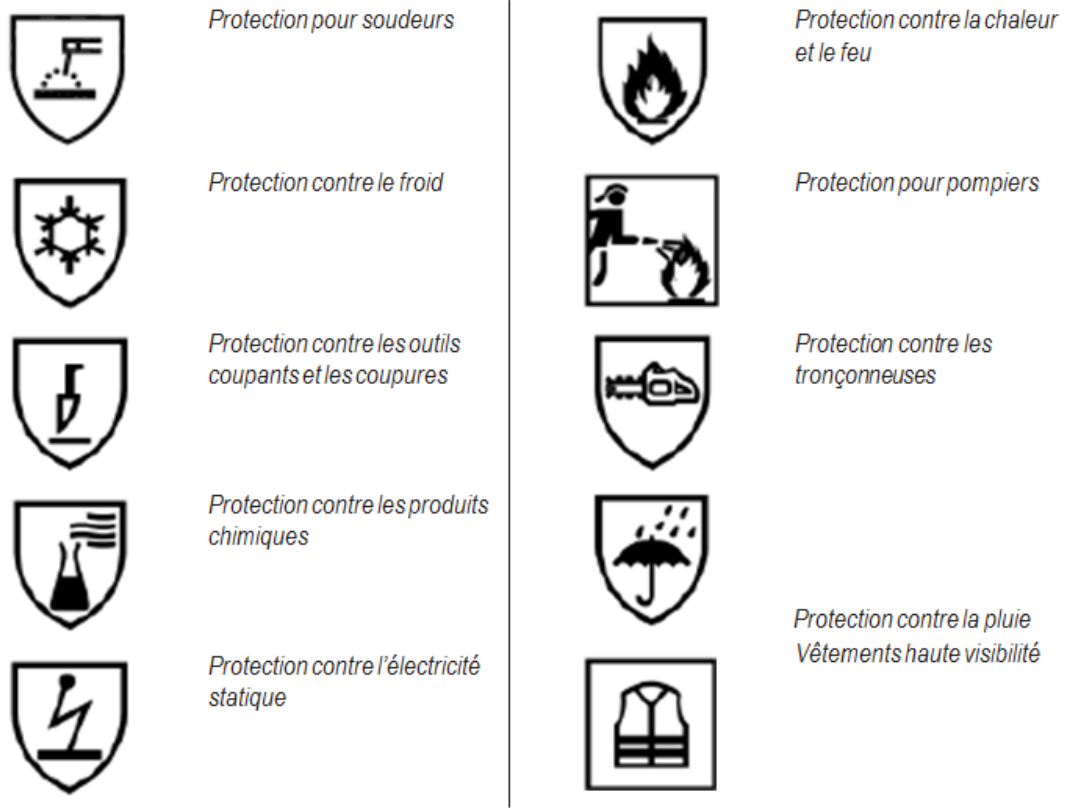
\includegraphics[width=0.75\textwidth]{images/vetements-protection.PNG}
\end{center}





\item \textbf{Définition incendie}: un incendie est une réaction chimique qui survient si trois éléments sont réunis:
\begin{itemize}
    \item une matière combustible,
    \item une matière comburante (ex: l’oxygène),
    \item une source d’inflammation.
\end{itemize}





\item \textbf{Définition:} Le Point d’éclair (Flash Point), aussi appelé "température d’inflammation" est la \textbf{température limite à laquelle un liquide combustible peut s’enflammer}.





\item \textbf{Définition:} la température d’auto-inflammation, aussi appelé point d'auto-inflammation est la température pour laquelle certaines matières peuvent s’enflammer spontanément, sans qu’il faille une flamme ou une étincelle (elle dépend de la matière).





\item \textbf{Définitions:}
\begin{itemize}
    \item Catalyseur : Produit qui influence la combustion (réaction combustible et oxygène).
    \item Catalyseur positif : Produit qui favorise la vitesse de réaction et donc attise le feu.
    \item Catalyseur négatif : Produit qui freine la vitesse de réaction et donc ralentit le feu.
\end{itemize}





\item Notions de UEL et LEL:
\begin{itemize}
    \item UEL = Upper Explosion Limit (= limite supérieure d'explosivité)
    \item LEL = Lower Explosion Limit (= limite inférieure d'explosivité)
\end{itemize}
\begin{center}
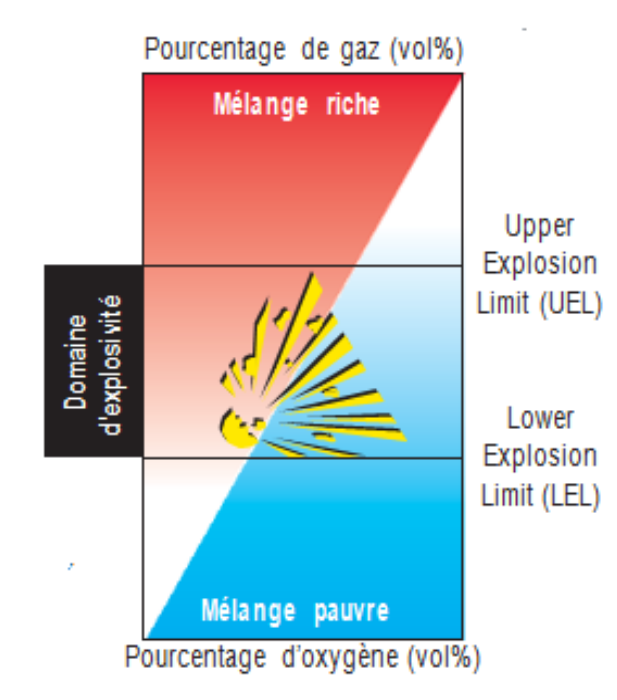
\includegraphics[width=0.5\textwidth]{images/uel-lel.PNG}
\end{center}
\begin{itemize}
    \item UEL = trop d'oxygène, pas assez de gaz
    \item LEL = trop de gaz, pas assez d'oxygène
\end{itemize}
\begin{center}
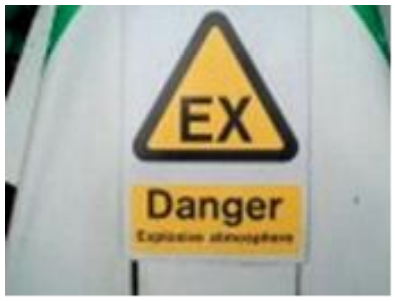
\includegraphics[width=0.3\textwidth]{images/risque-explosion.PNG}
\end{center}





\item Utiliser des outils/équipements anti-déflagrants afin d'éviter que les produits explosifs ne s'enflamment. Pictogramme:
\begin{center}

\includegraphics[width=0.2\textwidth]{images/antideflagrant.jpg}
\end{center}





\item Chaussures de sécurité anti-statiques:
\begin{itemize}
    \item Chaussures anti-statiques: résistance à l’életricité très basse, entre 0.1 et 1000 MegaOhm (M$ \Omega $).
    \item Chaussures ESD (ou ElectroStatic Discharge) ont une résistance électrique encore plus basse, entre 0.1 et 100 (M$ \Omega $).
\end{itemize}
Objectif: faible résistance $ \implies $ l'électricité passe dans le sol $ \implies $ pas de charges stockées dans le corps humain.
\begin{center}
\begin{tabular}{c c c}
    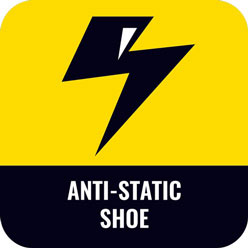
\includegraphics[width=0.2\textwidth]{images/chaussures-anti-statiques.jpg}
    &&
    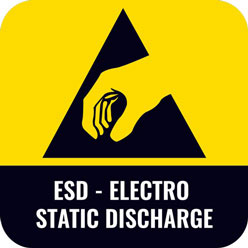
\includegraphics[width=0.2\textwidth]{images/chaussures-ESD.jpg}
\end{tabular}
\end{center}





\item Types de feux:
\begin{itemize}
    \item Classe A. Feux \textbf{secs} – Feux de solides SAUF le métal
    \begin{example}
        ex: bois, papier, coton, etc. \\
        Moyens d’extinction: eau, poudre d'extinction, couverture anti-feu
    \end{example}
    \item Classe B. Feux \textbf{gras} – Feux de liquides
    \begin{example}
        ex: essence, alcool, huile, etc. \\
        Moyens d’extinction: mousse, poudre d'extinction, sable (\textbf{jamais de l'eau})
    \end{example}
    \item Classe C. Feux de \textbf{gaz}
        \begin{example}
        ex: propane, butane, méthane, etc. \\
        Moyens d’extinction: couper l'arrivée de gaz, poudre, refroidir les environs et les bouteilles de gaz
    \end{example}
    \item Classe D. Feux de \textbf{métaux}
    \begin{example}
        ex: aluminium, potassium, sodium, etc. \\
        Moyens d’extinction: sable pour les petits feux, poudres spéciales sinon (\textbf{jamais de l'eau})
    \end{example}
    \item Classe E. Feux \textbf{non-classifiés}
    \begin{example}
        ex: feux d'origine électrique - court-circuit, surchauffe, etc. \\
        Moyens d’extinction: dioxyde de carbone ($ CO_2 $) ou une poudre appropriée
    \end{example}
    \item Classe F. Feux de \textbf{graisses}
    \begin{example}
        ex: produits de cuisson (huiles et graisses végétales ou animales) utilisés en cuisine. \\
        Moyens d’extinction: (\textbf{comme la classe B.}) mousse, poudre d'extinction, sable (\textbf{jamais de l'eau})
    \end{example}
\end{itemize}





\item \textcolor{red}{\textbf{Attention !}} Moyens d'extinction de feu:
\begin{center}
\begin{tikzpicture}
    \node[anchor=north west]{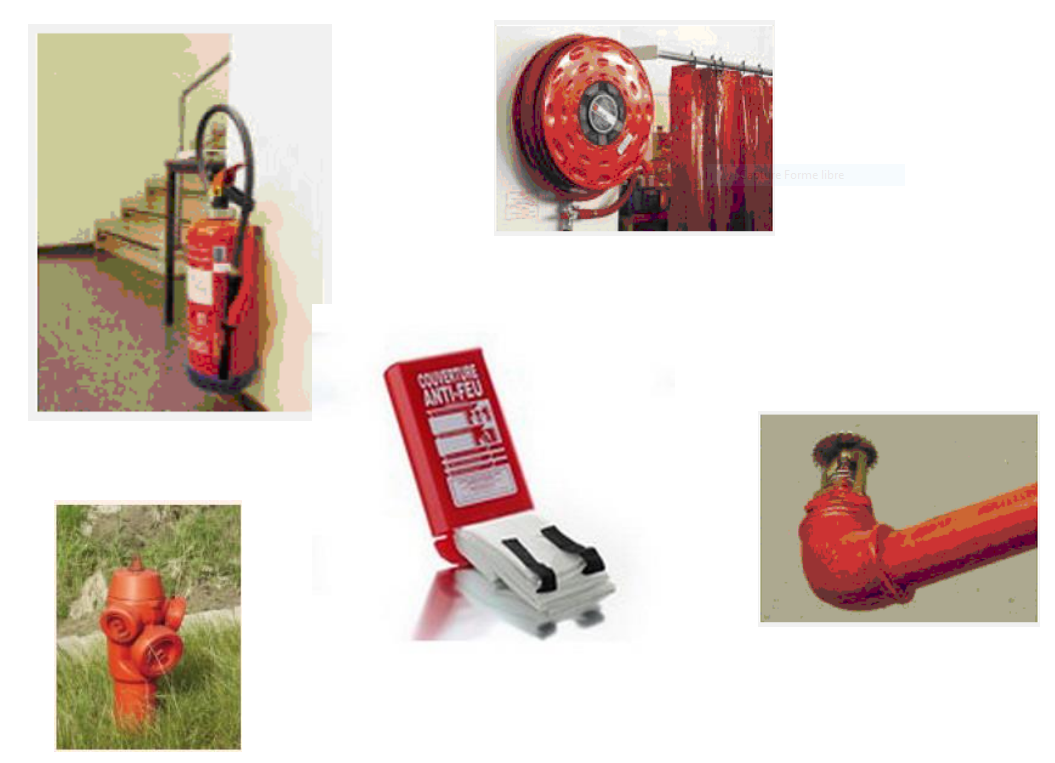
\includegraphics[width=15cm]{images/anti-incendie.PNG}};
    \node[anchor=north west] at (1,0.3) {extincteur ABC};
    \node[anchor=north west] at (8,0.3) {dévidoir};
    \node[anchor=north west] at (0.75,-11) {bouche d'incendie};
    \node[anchor=north west] at (6,-9.5) {couverture anti-feu};
    \node[anchor=north west] at (12,-9.25) {sprinkler};
\end{tikzpicture}
\end{center}





\item Manutention manuelle des charges:
\begin{itemize}
    \item En manutentionnant de lourdes charges ou en surchargeant le dos, on peut déplacer/abîmer les disques intervertébraux.
    \item Idéal = éviter la manutention.
    \item Pour prévenir les lésions, on doit utiliser les muscles les plus forts : les muscles des bras et des jambes.
\end{itemize}





\item Méthode de manutention correcte:
\begin{itemize}
    \item dos droit et le plus vertical possible,
    \item placer ses jambes le plus près possible de chaque côté de la charge,
    \item plier les genoux d’un peu moins de 90\textdegree,
    \item placer ses mains des 2 côtés de l'objet,
    \item remonter progressivement (jamais en une traite) et avec un dos droit en redressant les jambes,
    \item garder les bras tendus et le plus près possible du corps,
    \item déposer une charge se passe de la même façon en sens inverse,
    \item pour tourner, il faut déplacer les pieds et ne pas tourner le tronc.
\end{itemize}
Remarque: quand on est assis, il vaut mieux se lever avant de manutentionner des charges, sinon ce sont les muscles du dos qui travaillent.





\item Travailleuses enceintes: elles ne peuvent pas manutentionner des charges durant les trois derniers mois de leur maternité et durant la période de lactation.





\item Trébucher, tomber et glisser -- plus grands risques:
\begin{itemize}
    \item Sol glissant ou inégal;
    \item Différences de niveau;
    \item Carrelages, marches détachées, ...
    \item Saleté et déchets sur le sol;
    \item Accès encombrés;
    \item Courses dans les couloirs, les escaliers;
    \item Utiliser les rampes comme toboggan;
    \item Ne pas utiliser les rampes;
    \item Mauvaises semelles de chaussures.
\end{itemize}





\item \textcolor{red}{\textbf{Q. d'examen.}} Passages et voies de secours:
\begin{itemize}
    \item Les chemins d’entrée, de sortie et d’évacuation ont une largeur minimale de \textbf{80 cm},
    \item si il faut évacuer plus de 80 personnes, on ajoute 1 centimètre par personne,
    \item ex: 150 pers. $ \implies $ passage de 1 m 50.
\end{itemize}





\item Utilisation sûre de l’escalier:
\begin{itemize}
    \item Tenez fermement la rampe;
    \item Gardez les yeux fixes sur les marches;
    \item Ne portez pas de chaussures glissantes;
    \item Ne courez pas dans les escaliers;
    \item Ne portez rien qui gêne votre champ de vision;
    \item Attention aux marches de hauteur changeante;
    \item Laissez toujours la lumière allumée dans les escaliers;
    \item Ne jamais laisser traîner des objets sur l’escalier
\end{itemize}





\item Intensité d'éclairement:
\begin{itemize}
    \item 300 lux perception assez poussée des détails (travaux de bureau)
    \item 1000 lux perception extrêmement fine des détails (laboratoires, ateliers électroniques, etc.)
\end{itemize}
Remarques:
\begin{itemize}
    \item lux = intensité lumineuse.
    \item Il est important que les contrastes de lumière dans une pièce ne soient pas trop grands.
    \item La lumière ne doit pas arriver directement dans les yeux.
\end{itemize}





\item Le taux d’humidité relative de l’air doit être compris entre 40 \% et 70 \%. \\
Remarque: pour mesurer l'humidité de l'air, on utilise un \textbf{hygromètre} ($ \neq $ hydromètre).





\item \textcolor{red}{\textbf{Attention !}} Vitesse de l'air:
\begin{itemize}
    \item Pour les travaux légers, la vitesse de l’air est de 0,15 m/s (20 à 26 \textdegree C).
    \item Pour les travaux lourds, la vitesse de l’air peut être de 0,25 m/s.
\end{itemize}





\item La teneur en monoxyde de carbone recommandée se trouve entre 800 et 1500 ppm (parties par million).





\item \textcolor{red}{\textbf{Attention aux valeurs !}} Conditions sur les espaces de travail pour un bon rafraîchissement de l'air:
\begin{itemize}
    \item hauteur du local de travail = 2 m 50
    \item vitesse de l'air limitée à 0,5 m/s
    \item la taille du local correspond au nombre de personnes
    \item apport d’air frais et l’extraction de l’air vicié doit être de 30 $m^3$/h/personne
\end{itemize}





% \item Origines des risques psychosociaux:
% \begin{itemize}
%     \item L’organisation du travail (ex: les tâches, le style de management).
%     \item Le contenu du travail (ex: charge mentale/physique).
%     \item Les conditions de travail (ex: gestion des carrières, type d'horaire).
%     \item Les conditions de vie au travail (ex: bruit, éclairage).
% \end{itemize}





\item Différentes formes de harcèlement:
\begin{itemize}
    \item isoler socialement,
    \item rendre le travail désagréable ou impossible,
    \item ridiculiser.
\end{itemize}





\item Soutien (pour contrer le risque psychosocial):
\begin{itemize}
    \item possibilité de concertation, de participation,
    \item le travailleur a une responsabilité suffisante, reçoit un feedback régulier,
    \item bonnes conventions,
    \item présence d'une personne de confiance.
\end{itemize}





\item Différence entre harceler et taquiner: dans le cas du taquinement, il n’est pas question de systématisme et d’inégalité entre les parties.





\item Politique des courriels: un courriel doit rester strictement professionnel (pas d’insinuation, pas de taquinerie, etc.).





\end{itemize}















\section{Tome n\textdegree 2}





\begin{itemize}





\item \textcolor{red}{\textbf{Q. d'examen.}} RGIE = Réglement Général des Installations Électriques





\item Dangers de l'électricité:
\begin{center}
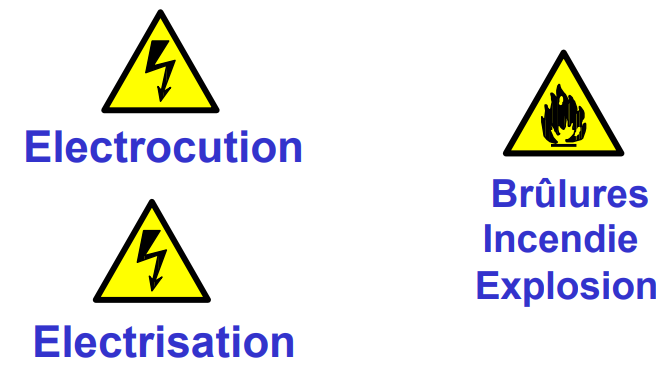
\includegraphics[width=0.3\textwidth]{images/elec01.PNG}
\end{center}
Remarques:
\begin{itemize}
    \item éléctrisation $ \neq $ éléctrocution
    \item électrisation = passage d'un courant électrique dans le corps d'un homme
    \item éléctrocution = action de causer une secousse mortelle par le passage d'un courant électrique
\end{itemize}





\item Classes du matériel:
\begin{center}
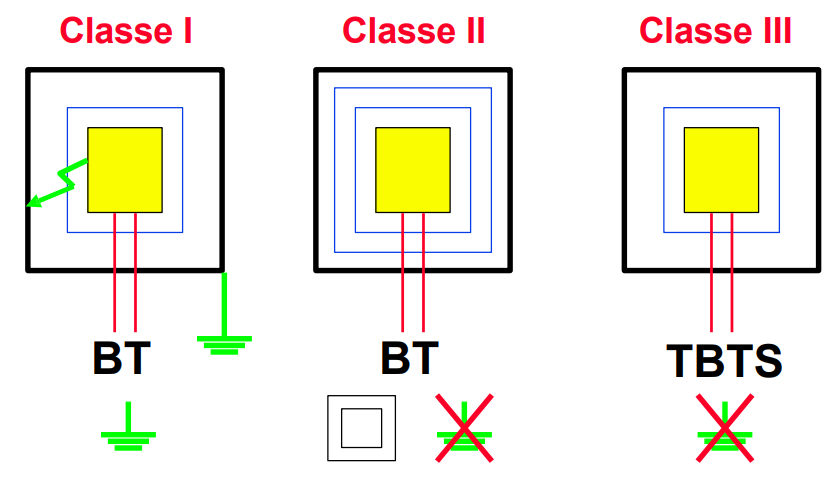
\includegraphics[width=0.5\textwidth]{images/elec02.PNG}
\end{center}
Remarques:
\begin{itemize}
    \item BT = basse tension
    \item TBTS = très basse tension de sécurité
    \item 
\begin{tikzpicture} \draw (0,0) -- (0,0.4) -- (0.4,0.4) -- (0.4,0) -- cycle; \draw (-0.1,-0.1) -- (-0.1,0.5) -- (0.5,0.5) -- (0.5,-0.1) -- cycle;
    \end{tikzpicture} \; = symbole de doule-isolation.
    \item 
\begin{tikzpicture} \draw (0,0) -- (0,0.2); \draw (0.1,0) -- (0.1,0.2); \draw (0.2,0) -- (0.2,0.2); \draw (-0.3,0.1) -- (0.1,-0.2) -- (0.5,0.1) -- (0.1,0.4) -- cycle;
    \end{tikzpicture} \; = symbole de TBTS.
    \item \begin{tikzpicture} \draw (0,0) -- (0,0.2); \draw (-0.3,0) -- (0.3,0); \draw (-0.2,-0.1) -- (0.2,-0.1); \draw (-0.1,-0.2) -- (0.1,-0.2);
    \end{tikzpicture} \; = symbole de prise de terre.
\end{itemize}
\begin{center}
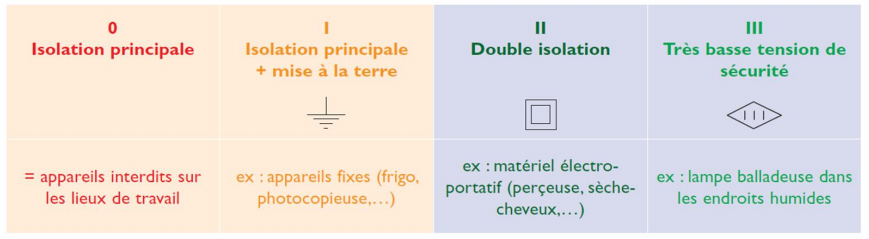
\includegraphics[width=0.95\textwidth]{images/elec03.PNG}
\end{center}





\item \textcolor{red}{\textbf{Attention !}}
\begin{center}
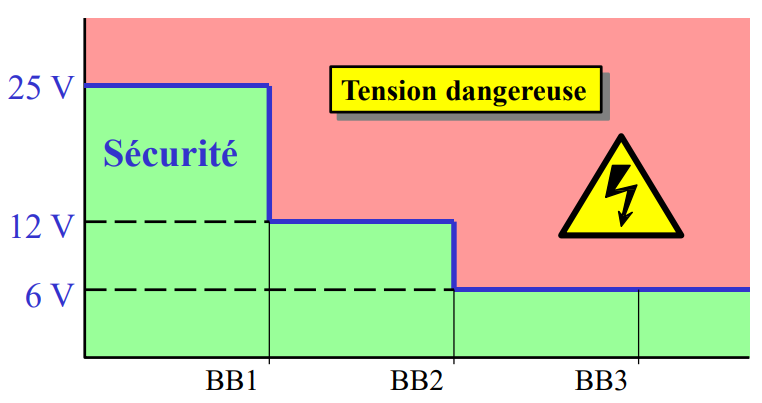
\includegraphics[width=0.75\textwidth]{images/elec04.PNG}
\end{center}
Remarques:
\begin{itemize}
    \item Toucher sans danger peut se faire en TBTS.
    \item BB1 = mains sèches.
    \item BB2 = mains moites.
    \item BB3 = mains mouillées.
\end{itemize}





\item Les 7 règles d’or pour assurer un travail hors tension (sur une installation éléctrique):
\begin{itemize}
    \item Préparer les travaux
    \item Séparer
    \item S’assurer contre la réalimentation
    \item Contrôler l’absence de tension
    \item Mettre à la terre, décharger et mettre en courtcircuit
    \item Baliser et/ou protéger
    \item Mettre à disposition
\end{itemize}





\item \textcolor{red}{\textbf{Attention !}}
\begin{center}
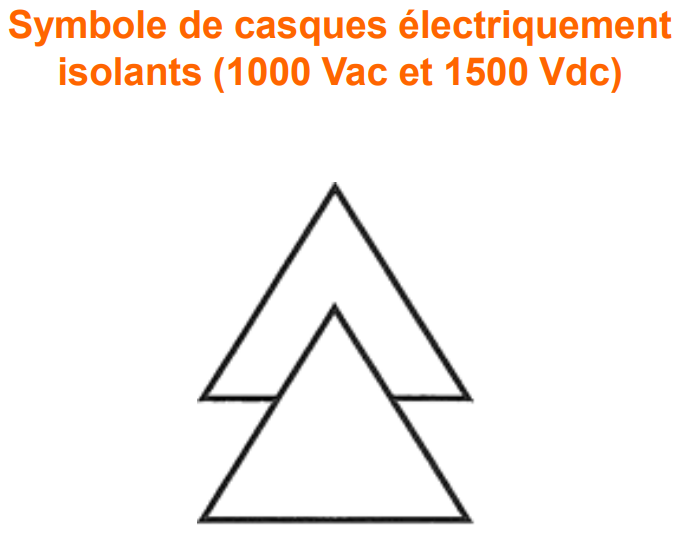
\includegraphics[width=0.4\textwidth]{images/elec05.PNG}
\end{center}





\item Qu'est-ce ?
\begin{center}
\begin{tabular}{cc}
    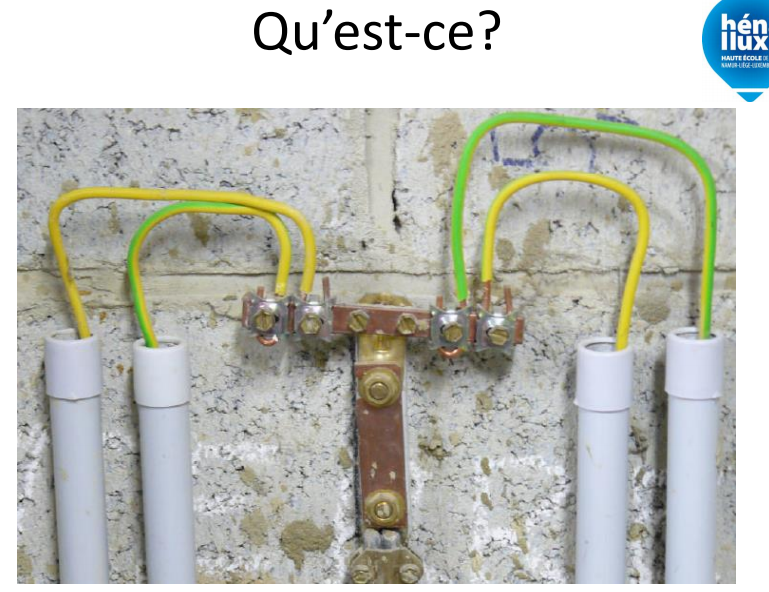
\includegraphics[width=0.4\textwidth]{images/elec06.PNG}
    &
    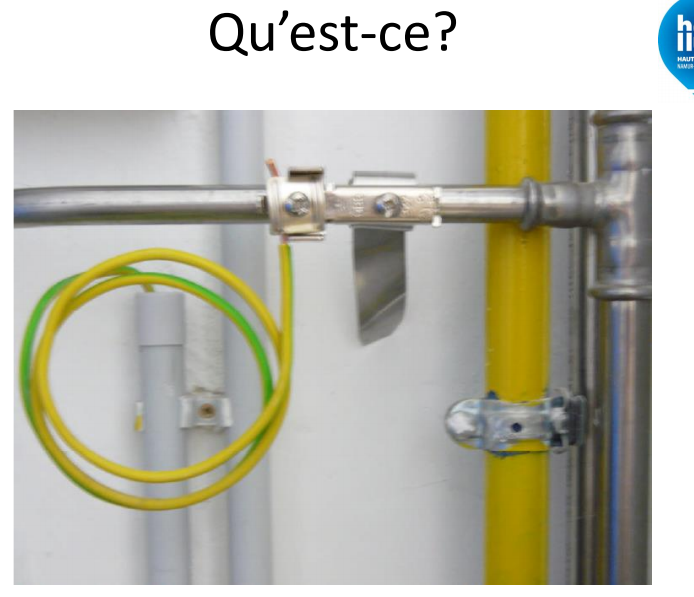
\includegraphics[width=0.4\textwidth]{images/elec07.PNG}
    \\
    Prise de terre
    &
    Relier la conduite d'eau à la terre
\end{tabular}
\end{center}





\item Éléctricité statique:
\begin{center}
    \begin{tabular}{cc}
        
\includegraphics[width=0.2\textwidth]{images/elec08.PNG}
        &
        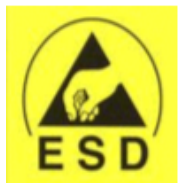
\includegraphics[width=0.2\textwidth]{images/elec09.PNG}
        \\
        ESD Susceptible
        &
        ESD Protective
        \\
        éléments à \textbf{risques} électrostatiques
        &
        produits \textbf{protégeant} des décharges électrostatiques
    \end{tabular}
\end{center}





\item \textbf{Définitions}:
\begin{itemize}
    \item produit cancérigène = produit pouvant augmenter le risque de cancer
    \item produit mutagène = produit pouvant causer des mutations génétiques
    \item produit tératogène = produitpouvant attaquer la reproductabilité et/ou dommageable pour le foetus
    \item dose = quantité de produits dangereux qui est absorbée par l’organisme durant une certaine période
    \item effet aigu = immédiatement évident (ex: perte de connaissance)
    \item effet chronique =  évident après une exposition de longue durée a de basses concentrations
    \item toxicité = le pouvoir d'un produit d’occasionner un dommage au corps humain
\end{itemize}





\item Oxygène:
\begin{itemize}
    \item l'atmosphère contient 21 \% d'$ O_2 $
    \item l'homme a besoin d'air avec minimum 18 \% d'$ O_2 $
    \item dans un local, au moins 19 \% d'$ O_2 $ doit toujours être garanti
\end{itemize}





\item Danger monoxyde de carbone: ce gaz n’a pas de goût, pas d’odeur et pas de parfum et ne peut pas être détecte par l’homme. C’est pourquoi on l’appelle le tueur silencieux.





\item \textcolor{red}{\textbf{Attention !}} L’informatique se met au vert:
\begin{itemize}
    \item ROHS (restriction of the use of certain hazardous substances in electrical and electronic equipment): contrôle l’utilisation des substances dangereuses.
    \item DEEE (déchets d’équipements électriques et électroniques): rend les producteurs responsables de la reprise, du traitement et de l’élimination non polluante des déchets électroniques.
\end{itemize}





\item Signaux:

\end{itemize}

\begin{center}
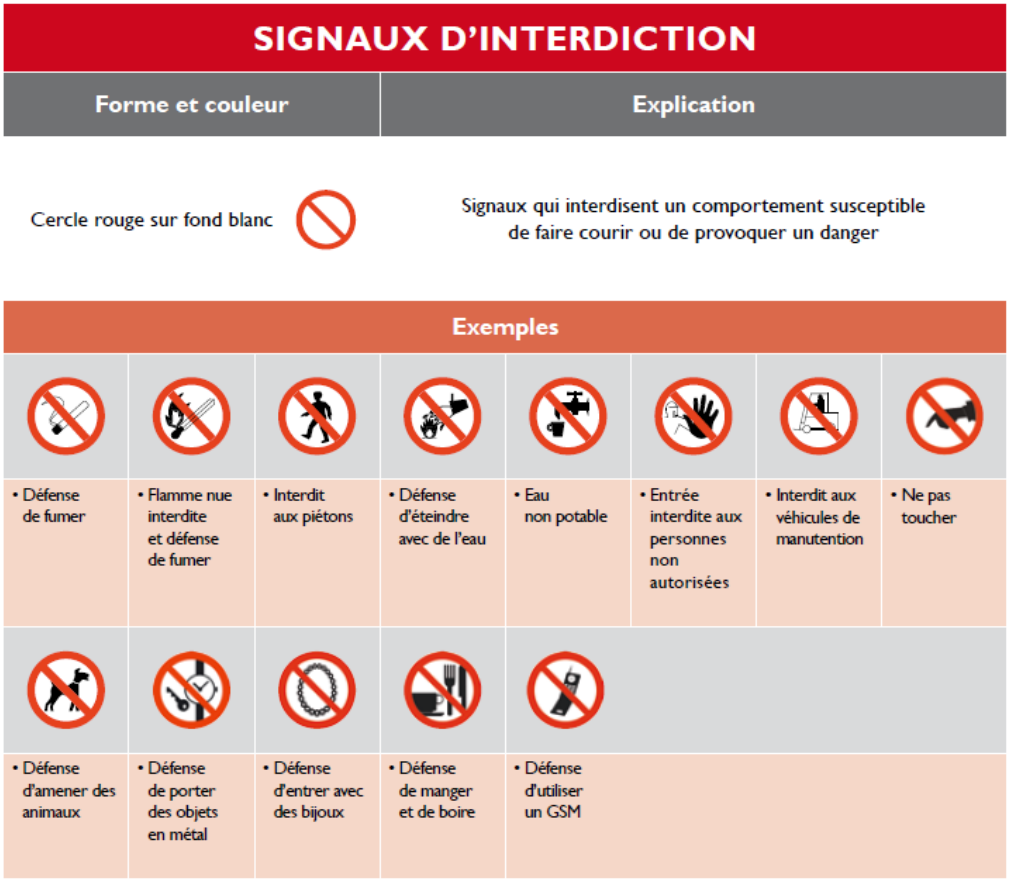
\includegraphics[width=0.95\textwidth]{images/signaux1.PNG}
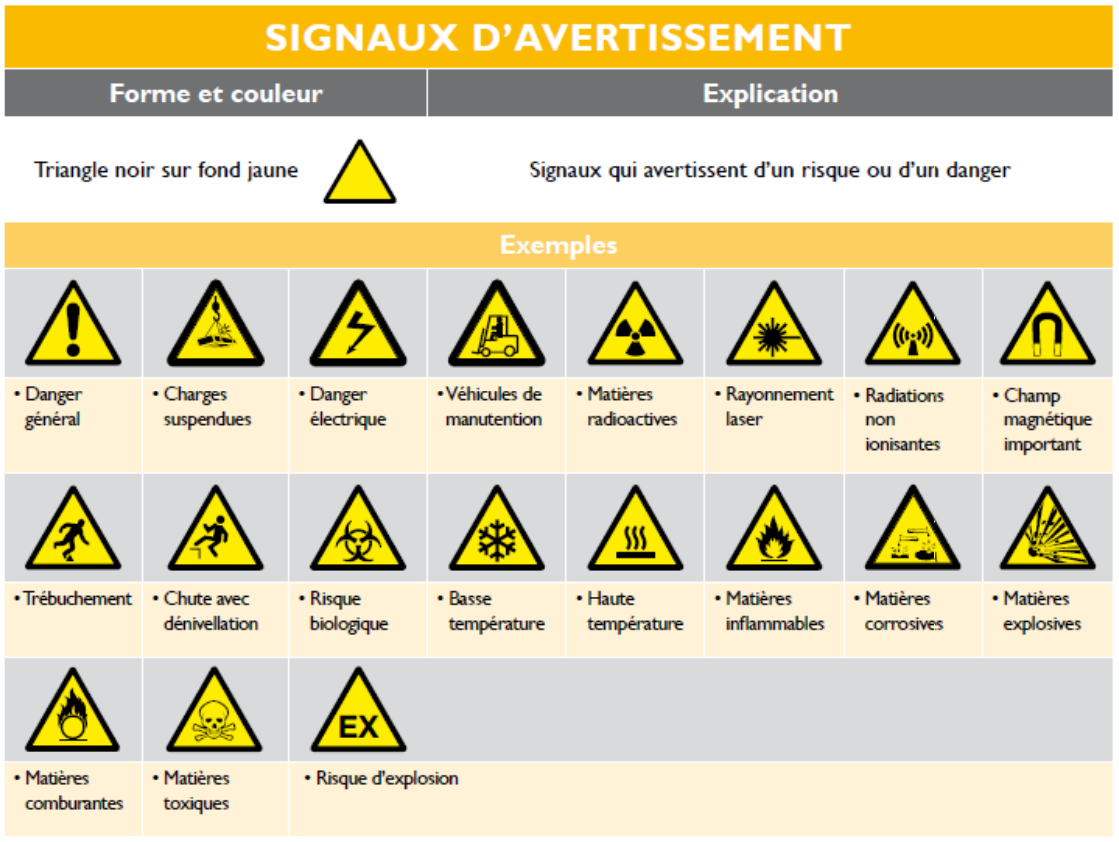
\includegraphics[width=0.95\textwidth]{images/signaux2.PNG}
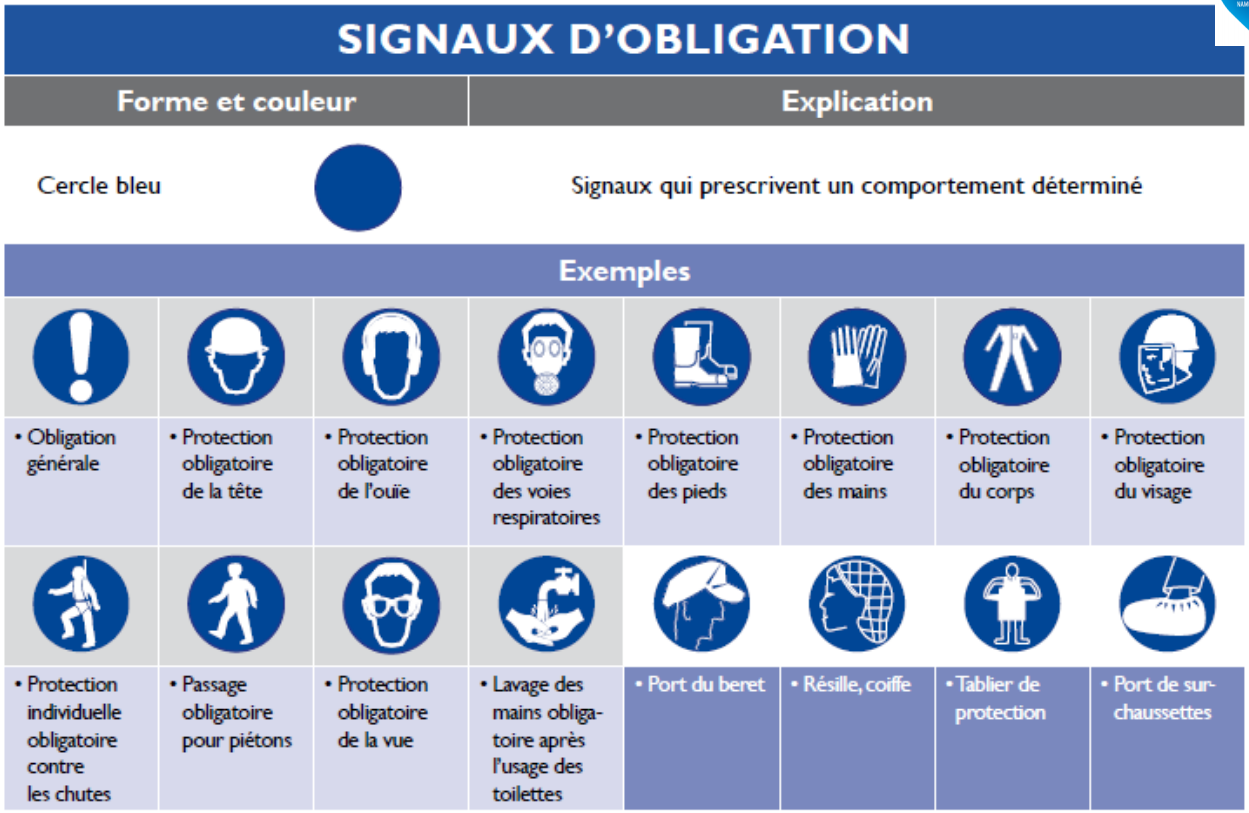
\includegraphics[width=0.95\textwidth]{images/signaux3.PNG}
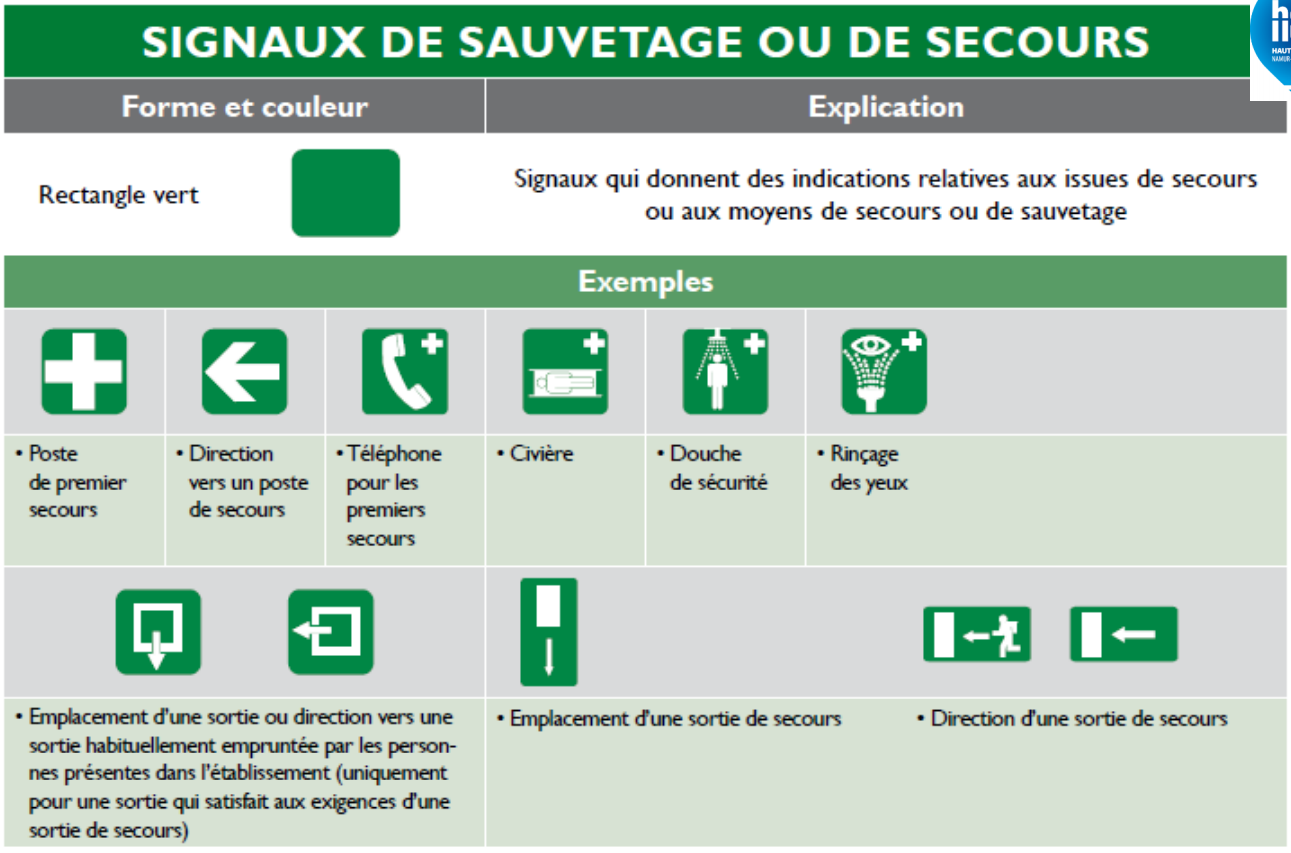
\includegraphics[width=0.95\textwidth]{images/signaux4.PNG}
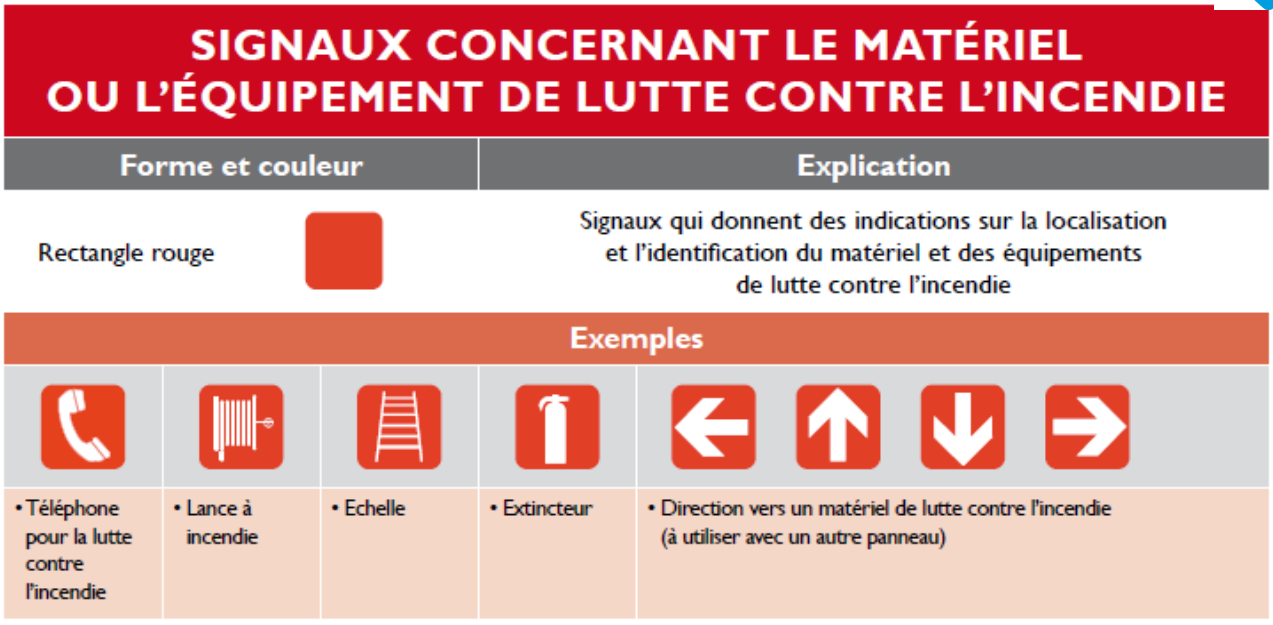
\includegraphics[width=0.95\textwidth]{images/signaux5.PNG}
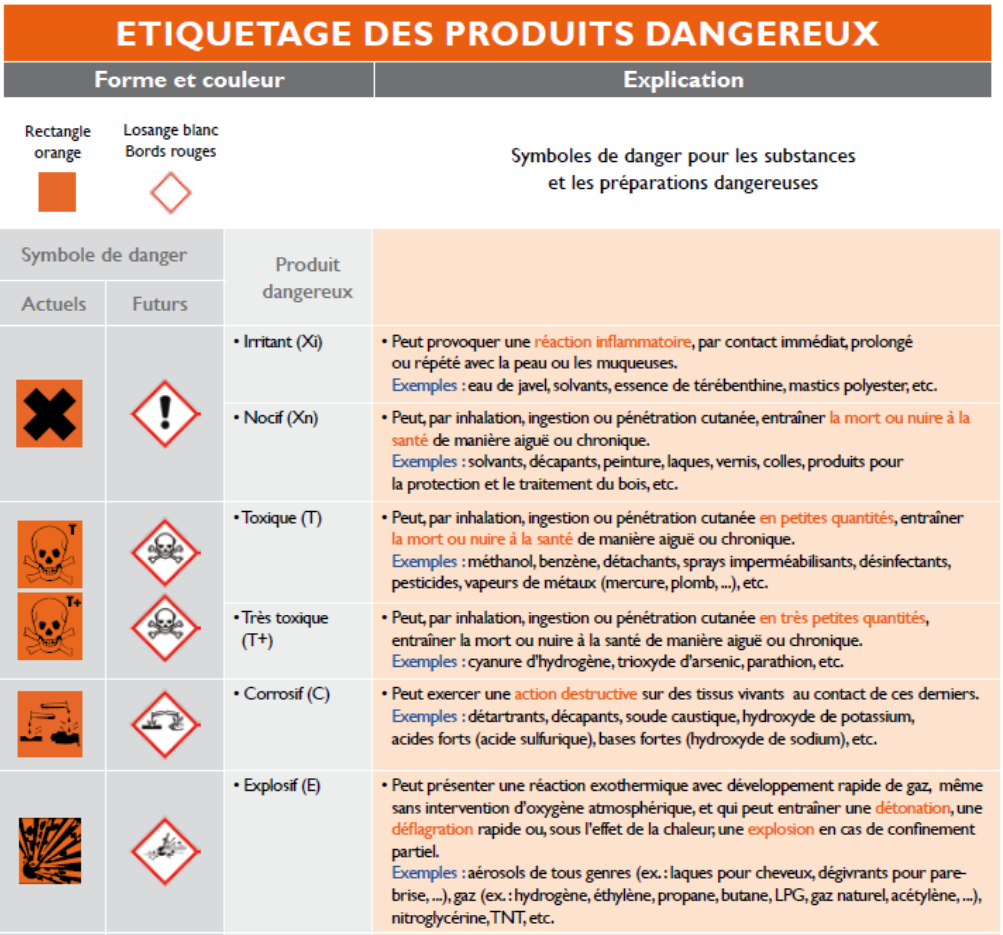
\includegraphics[width=0.95\textwidth]{images/signaux6.PNG}
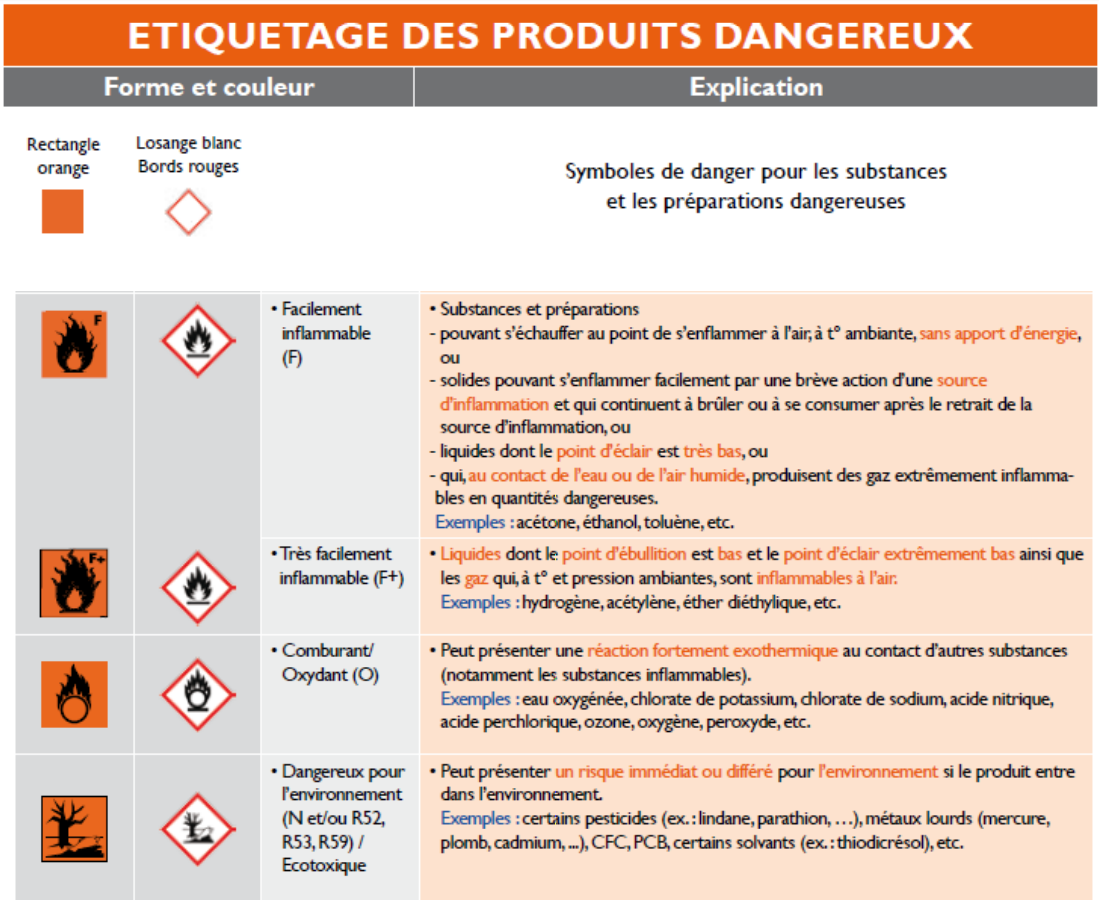
\includegraphics[width=0.95\textwidth]{images/signaux7.PNG}
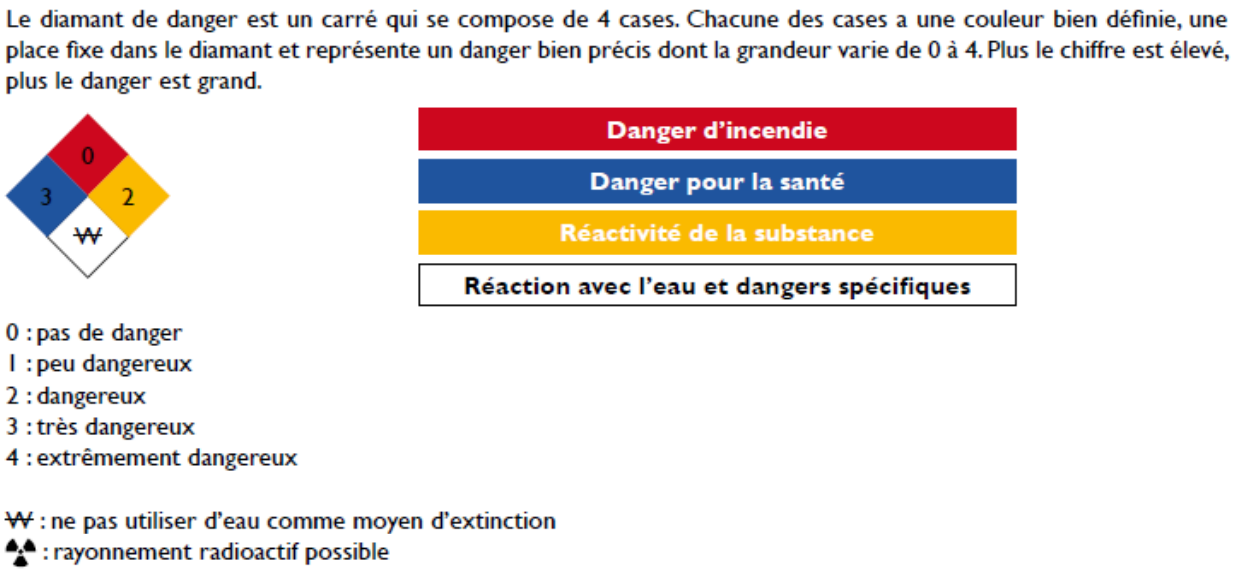
\includegraphics[width=0.95\textwidth]{images/signaux8.PNG}
\end{center}















\appendix \newpage















\import{./}{annexes.tex}





\end{document}
